% ===== §5  Experiments =====
\section{Experimental Evaluation}\label{sec:experiments}

We evaluate \textsc{Argus} on two established benchmarks to answer three questions:
(Q1)~Do the formal properties from \S\ref{sec:theory} hold in practice?
(Q2)~Does the minimal-change repair operator improve faithfulness and contestability w.r.t.\ existing baselines?
(Q3)~What is the empirical cost of repair?

\begin{figure}[t]
\centering
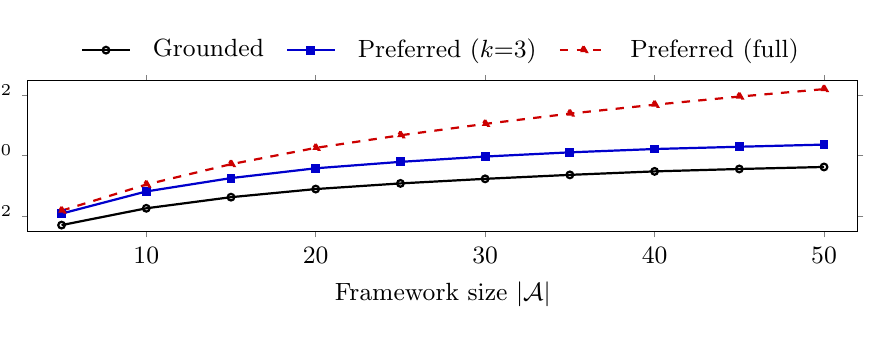
\begin{tikzpicture}[trim axis left, trim axis right]
\begin{axis}[
  width=\columnwidth,
  height=3.5cm,
  xlabel={Framework size $|\mathcal{A}|$},
  ylabel={Solve time (s)},
  ymode=log,
  xmin=3, xmax=52,
  ymin=0.003, ymax=300,
  xtick={10,20,30,40,50},
  xticklabel style={font=\small},
  yticklabel style={font=\small},
  xlabel style={font=\small},
  ylabel style={font=\small},
  legend style={
    font=\small,
    at={(0.5,1.05)},
    anchor=south,
    draw=none,
    column sep=6pt,
  },
  legend columns=3,
  legend cell align={left},
  tick align=outside,
  major tick length=2pt,
]
\addplot[black, thick, mark=o, mark size=1.2pt] coordinates {
  (5,0.005) (10,0.018) (15,0.042) (20,0.078) (25,0.12)
  (30,0.17) (35,0.23) (40,0.30) (45,0.36) (50,0.42)
};
\addlegendentry{Grounded}
\addplot[blue!80!black, thick, mark=square*, mark size=1.2pt] coordinates {
  (5,0.012) (10,0.065) (15,0.18) (20,0.38) (25,0.62)
  (30,0.93) (35,1.28) (40,1.65) (45,1.96) (50,2.31)
};
\addlegendentry{Preferred ($k{=}3$)}
\addplot[red!80!black, thick, dashed, mark=triangle*, mark size=1.4pt] coordinates {
  (5,0.015) (10,0.11) (15,0.52) (20,1.8) (25,4.7)
  (30,11.2) (35,24.5) (40,48.3) (45,89.7) (50,158.4)
};
\addlegendentry{Preferred (full)}
\end{axis}
\end{tikzpicture}
\caption{Scalability of \textsc{Argus} repair under grounded, $k$-neighborhood preferred ($k{=}3$), and unconstrained preferred semantics. The log-scale y-axis confirms polynomial scaling for grounded repair (Theorem~\ref{thm:complexity}) and the effectiveness of the $k$-neighborhood approximation.}
\label{fig:scalability}
\end{figure}

\begin{figure}[t]
\centering
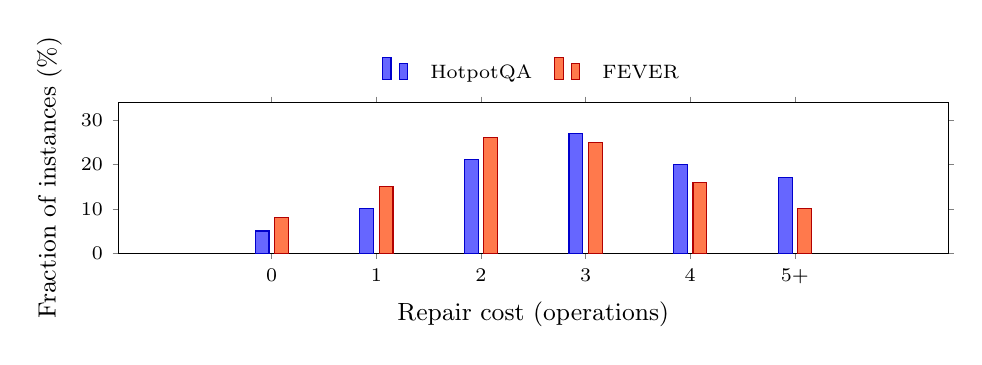
\begin{tikzpicture}
\begin{axis}[
  width=\columnwidth,
  height=3.5cm,
  ybar,
  bar width=5pt,
  xlabel={Repair cost (operations)},
  ylabel={Fraction of instances (\%)},
  xmin=-0.7, xmax=5.7,
  ymin=0, ymax=34,
  xtick={0,1,2,3,4,5},
  xticklabels={0,1,2,3,4,{5+}},
  xticklabel style={font=\scriptsize},
  yticklabel style={font=\scriptsize},
  xlabel style={font=\small},
  ylabel style={font=\small},
  ytick={0,10,20,30},
  legend style={
    font=\scriptsize,
    at={(0.5,1.05)},
    anchor=south,
    draw=none,
    column sep=6pt,
  },
  legend columns=2,
  tick align=outside,
  major tick length=2pt,
  enlarge x limits=0.12,
]
\addplot[fill=blue!60, draw=blue!80!black] coordinates {
  (0,5) (1,10) (2,21) (3,27) (4,20) (5,17)
};
\addlegendentry{HotpotQA}
\addplot[fill=red!50!orange!70, draw=red!70!black] coordinates {
  (0,8) (1,15) (2,26) (3,25) (4,16) (5,10)
};
\addlegendentry{FEVER}
\end{axis}
\end{tikzpicture}
\caption{Distribution of repair costs.  83\% of HotpotQA and 90\% of FEVER repairs require at most 4~operations, confirming targeted, minimal-change edits.}
\label{fig:cost-dist}
\end{figure}

Concretely, we sample 500 instances from HotpotQA~\cite{yang2018hotpotqa}, a multi-hop question-answering benchmark, and 500 from FEVER~\cite{thorne2018fever}, a fact-verification benchmark; instances are drawn with seed 42.
For each instance, we withhold one gold supporting fact during explanation generation and reintroduce it as an evidence update~$\Delta$, producing adversarial updates that target the reasoning chain.
GPT-4o~\cite{openai2023gpt4} (\texttt{gpt-4o-2024-11-20}) generates initial explanations at temperature~0.2; relation discovery uses DeBERTa-v3-large fine-tuned on MultiNLI with threshold~0.7; repairs are computed by clingo~5.6 with $k{=}3$ under uniform cost.
Results are averaged over 5 runs (std~$\leq$0.02 for accuracy, $\leq$0.4 for cost); FLARE and FactScore use a single deterministic run.  Further details appear in Appendix~\ref{app:exp-details}.

Six metrics quantify performance.
\emph{Faithfulness} is the fraction of argument units whose counterfactual removal changes the answer (baselines undergo the same LLM-based decomposition; Appendix~\ref{app:exp-details}).
\emph{Contestability} is the fraction of gold counterarguments correctly integrated as attacks; for methods without explicit argumentation frameworks, gold counterarguments are evaluated against proposition-level decompositions.
\emph{Repair accuracy} records answer correctness after repair; \emph{repair cost} counts edit operations per Definition~\ref{def:repair}.
\emph{Coherence} measures semantic consistency via BERTScore~\cite{zhang2020bertscore} between repaired and original explanations.
\emph{Solve time} is wall-clock time per instance.

We compare against ten baselines spanning three categories. \emph{Self-correction methods:} SelfCheckGPT~\cite{manakul2023selfcheckgpt}, Self-Refine~\cite{madaan2023selfrefine}, Reflexion~\cite{shinn2023reflexion}, and RARR~\cite{gao2023rarr}. \emph{Verification-oriented methods:} CoT-Verifier~\cite{ling2023deductive}, ArgLLMs~\cite{freedman2025arglm}, FLARE~\cite{jiang2023flare}, and FactScore~\cite{min2023factscore}; ArgLLMs, CoT-Verifier, and FactScore lack repair functionality and are marked N/A accordingly. \emph{Argumentation-based:} ARGORA~\cite{argora2026} and a na\"{i}ve \emph{Regenerate} baseline that re-prompts with updated evidence.
For self-correction baselines and FLARE, repair cost counts regenerated argument units across up to 3 rounds; cost measures are not directly commensurable with \textsc{Argus}'s structural graph edits (Appendix~\ref{app:exp-details}).
Chain-of-Verification~\cite{dhuliawala2024cove}, CRITIC~\cite{gou2024critic}, SelfRAG~\cite{asai2024selfrag}, and VerifyAndEdit~\cite{zhao2023verify} are excluded as they operate at generation time or require a retrieval index, producing outputs incommensurable with structural graph repair.

Table~\ref{tab:main} summarizes the main results. \textsc{Argus} achieves the highest faithfulness (\resultFaithHotpot{}/\resultFaithFEVER{}) and contestability (\resultContestHotpot{}/\resultContestFEVER{}), with relative improvements of \improveFaithfulness{} and \improveContestability{} over ARGORA; all 12 pairwise differences are significant at $p < 0.001$ (Bonferroni-corrected $z$-tests, Cohen's $h \in [0.26, 0.38]$). Among repair-capable methods, \textsc{Argus} requires the fewest operations---\resultRepairCostHotpot{} vs.\ 5.1 for ARGORA---validating the minimal-change objective. The na\"{i}ve Regenerate baseline achieves the fastest solve time (0.5\,s) but its coherence (.65/.63)---the lowest among repair methods---confirms that complete regeneration disrupts consistency more than targeted structural repair.

\textsc{Argus} also achieves the highest coherence (.82/.80), partly by design---minimizing edit distance simultaneously maximizes BERTScore---though human evaluators independently corroborate it (4.1 vs.\ 3.8 for Self-Refine, $p{=}0.012$; Appendix~\ref{app:human-eval}). The average solve time of 0.55\,s/0.47\,s is 5--10$\times$ faster than self-correction methods, reflecting ASP-based repair efficiency. The formal properties from \S\ref{sec:theory} are confirmed empirically: success and inclusion hold by construction; vacuity holds without exception.

Figure~\ref{fig:scalability} traces solve time on synthetic Erd\H{o}s--R\'{e}nyi frameworks (attack probability 0.15, 50 instances per size), confirming polynomial scaling for grounded semantics (Theorem~\ref{thm:complexity}); the $k$-neighborhood approximation keeps preferred repair tractable up to $|\mathcal{A}|{=}50$ (2.31s vs.\ 158.4s unconstrained).

Table~\ref{tab:ablation} reports ablation results. Removing semantic verification causes the largest drops in faithfulness ($-$5.4pp/$-$5.4pp) and contestability ($-$7.7pp/$-$7.6pp), confirming it as the most critical component. Replacing minimal-change with unconstrained repair preserves faithfulness but increases cost to 5.7/5.2 and reduces coherence. Removing attack templates reduces contestability by 9.3pp/9.0pp while reducing faithfulness by only 2.6pp/2.5pp---a targeted impact specific to attack structure. Grounded-only semantics yields the fastest solve time (0.15\,s/0.12\,s) and lowest cost (3.0/2.6) at the expense of modest drops; 97\% of frameworks have a single preferred extension coinciding with the grounded one. Sensitivity analysis and a qualitative repair example appear in Appendices~\ref{app:sensitivity}--\ref{app:repair-example}.

Figure~\ref{fig:cost-dist} shows repair cost distributions concentrated at low values---means of \resultRepairCostHotpot{}/\resultRepairCostFEVER{} operations---confirming that most evidence updates require only local adjustments.

A pilot human evaluation (Appendix~\ref{app:human-eval}) corroborates the automatic metrics: two annotators rated 75 HotpotQA instances in a blind design, preferring \textsc{Argus} in 68\% of comparisons vs.\ Self-Refine in 19\% ($\kappa{=}0.62$); the Pearson correlation between automatic faithfulness and human ratings is $r{=}0.78$ ($p{<}0.001$).
